\section{Geometric constraints on cones and  silhouette lines}
\label{sec:constraints}

Following~\cite{gummeson22pose, gummeson24relative}, we briefly recall some geometric properties of cylinders and their image projections, which form the basis for the constraints in our systems. A cylinder $\mathcal{C}$ can be interpreted as a cone with its vertex $\mathbf{V}$ lying on the plane at infinity. Algebraically, both cones and cylinders are represented by a singular quadric surface with matrix $\mathsf{Q}$ such that a point $\mathbf{X}$ belongs to $\mathcal{C}$ if and only if $\mathbf{X}^\top \mathsf{Q} \mathbf{X} = 0$.

A cylinder is a generate quadric and as such the rank of it's matrix $\mathsf{Q}$ is not full. The vertex $\mathbf{V}$ lies in the null-space of $\mathsf{Q}$, that is, $\mathsf{Q} \mathbf{V} = \mathbf{0}$. For cylinders, this vertex takes the form $\mathbf{V} = {(\mathbf{w}, 0)}^\top$ in homogeneous coordinates, where $\mathbf{w}$ defines the direction of the cylinder’s axis.

\paragraph{}
Rather than working directly with $\mathsf{Q}$, it is convenient to use the dual quadric $\mathsf{Q}^* = \mathsf{Q}^{-1}$, which encodes the set of all planes tangent to $\mathcal{C}$. See Figure~\ref{fig:quadric_surface_dual}

Technically speaking, all planes containing $\mathbf{V}$ are tangent to $\mathsf{Q}$ but not all of them uniquely define the surface $\mathsf{Q}^*$. See Figure~\ref{fig:cone_plane_singlepoint}.
To uniquely identify the dual quadric $\mathsf{Q}^*$ in terms of the tangent planes two conditions must be satisfied:
\begin{equation}
\begin{cases}
\Pi^\top \mathsf{Q}^* \Pi = 0, \\
\Pi^\top \mathbf{V} = 0.
\end{cases}
\end{equation}

These two conditions can be formulated in terms of silhouette lines $l^h$. The backprojection of each silhouette line, given by $\mathsf{P}^\top l^h$, defines a 3D plane that is tangent to the cylinder $\mathcal{C}$ and passes through the camera center. Moreover, since this tangent plane is  aligned with the axis of the cylinder, $\mathsf{P}^\top l^h$ must contain the point at infinity $\mathbf{V}$ corresponding to the direction of the cylinder's axis. 
As a result, each visible silhouette line $l^h$ induces two constraints on the camera parameters of the form:

\begin{align}
l^{h \top} \mathsf{P} \mathsf{Q}^* \mathsf{P}^\top l^h &= 0 \label{eq:dual_quadric_constraint} \\
l^{h \top} \mathsf{P} \mathbf{V} &= 0.\label{eq:vertex_constraint}
\end{align}

\begin{figure}[hb]
		\centering
		\subfloat[
				The plane envelop of a dual quadric $\mathsf{Q}^*$. Tangent planes $\Pi_i$ define the overall surface
			]{
			\begin{tikzpicture}[scale=0.9, every node/.style={font=\large, transform shape}]
				% Include the image
				\node[anchor=south west,inner sep=0] (img) at (0,0) {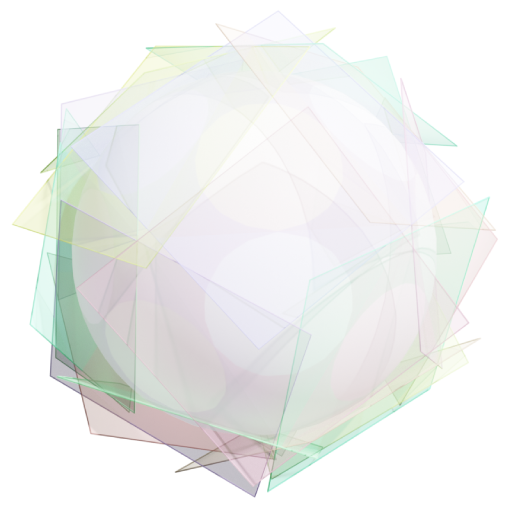
\includegraphics[width=0.5\textwidth]{images/quadric_surface_dual}};
				\begin{scope}[x={(img.south east)},y={(img.north west)}]
					\node at (0.8,0.14) {$\mathsf{Q}^*$};
					\node at (0.20,0.47) {$\Pi_1$};
					\node at (0.55,0.38) {$\Pi_2$};
					\node at (0.75,0.75) {$\Pi_3$};
				\end{scope}
				\label{fig:quadric_surface_dual}
			\end{tikzpicture}
		}
		\hspace{1cm}
		\subfloat[
			An example of a plane $\Pi$ tangent to a cone $\mathcal{C}$, which does not define the quadric surface $\mathsf{Q}^*$
		]{
			\begin{tikzpicture}[scale=0.9, every node/.style={font=\large, transform shape}]
				% Include the image
				\node[anchor=south west,inner sep=0] (img) at (0,0) {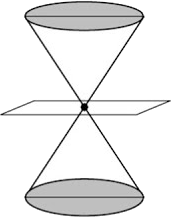
\includegraphics[width=0.35\textwidth]{images/cone_plane_singlepoint}};
				\begin{scope}[x={(img.south east)},y={(img.north west)}]
					\node at (0.20,0.42) {$\Pi$};
					\node at (0.8,0.28) {$\mathsf{Q}^*$};
					\node at (0.58,0.5) {$\mathbf{V}$};
				\end{scope}
				\label{fig:cone_plane_singlepoint}
			\end{tikzpicture}
		}
\end{figure}